\newpage
\subsection{BindingDB}
BindingDB \cite{gilson2016bindingdb} is an online database of drug-target interactions and measured binding affinity values. As of February 2021, BindingDB contains 41,328 entries with DOI, 2,114,159 binding affinity data for 928,022 small molecules, and 8,202 protein targets. Binding affinity is usually expressed in measures such as inhibition constant ($K_i$), dissociation constant ($K_d$), and the half-maximal inhibitory concentration (IC50). For that purpose, 2,077,458 $K_i$ (nM), $K_d$ (nM), and IC50 (nM) values were compiled from the database within the scope of the thesis. 

To benchmark the performance of graph-based representational learning, we use BDB dataset \cite{ozccelik2021chemboost} that is filtered from the BindingDB database. 24,404 binding affinities were observed for all pairs of 924 ligand and 480 proteins, measured by the $pK_d$ value (log-transformed kinase dissociation constant) \cite{ozccelik2021chemboost}. $pK_d$ correlates positively with the binding strength, and the value varies between 1.6 and 13.3. The number of ligands with strong binding affinity values is 3,428 (\textit{i.e.}, $pK_d \geq 7$) according to literature \cite{he2017simboost}. Figure \ref{fig:bdb} illustrates the distribution of the binding affinity values of proteins - ligand pairs in the BDB dataset. 
\begin{figure}
    \centering
        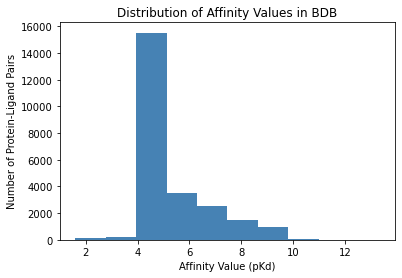
\includegraphics[width=0.5\linewidth]{chapters/materials_and_methods/datasetpreparation/figures/bdb.png} 
    \caption{Distribution of binding affinity values in BDB.}
    \label{fig:bdb}
\end{figure}

%BDB dataset consists of 5 different setups for training and evaluating the model performance. To evaluate the performance of DeepDTA, we trained the DeepDTA model with the knowledge derived from heterogeneous networks on five training setups of BDB dataset \cite{ozccelik2021chemboost}, and tested the models in the corresponding test sets. 